%%%%%%%%%%%%%%%%%%%%%%%%%%%%%%%%%%%%%%%%%%%%%%%%%%%%%%%%%%%%%%%%%%%%%%%%%%%%%%%%%
\subsection{FCT Scheme}
%%%%%%%%%%%%%%%%%%%%%%%%%%%%%%%%%%%%%%%%%%%%%%%%%%%%%%%%%%%%%%%%%%%%%%%%%%%%%%%%%
\begin{frame}
\frametitle{FCT Antidiffusive Flux Definition}

\begin{itemize}
   \item Recall that FCT defines antidiffusive correction fluxes
      from a low-order, monotone scheme to a high-order scheme. Calling
      these fluxes $\correctionfluxvector$, this gives
      \begin{equation}
        \lumpedmassmatrix\frac{
          \textcolor{secondarycolorheavy}{\solutionvector^{H}}
            -\solutionvector^n}{\dt}
          + (\ssmatrix+\diffusionmatrix^L)\solutionvector^n = \ssrhs^n
          + \textcolor{secondarycolorheavy}{\correctionfluxvector} \eqp
      \end{equation}
   \item Subtracting the high-order scheme equation from this gives the
      definition of $\correctionfluxvector$:
      \begin{equation}
        \correctionfluxvector \equiv
          -(\consistentmassmatrix-\lumpedmassmatrix)
          \frac{\solutionvector^{H}-\solutionvector^n}{\dt}
          + (\diffusionmatrix^L-\diffusionmatrix^{H,n})\solutionvector^n \eqp
      \end{equation}
   \item Decomposing $\correctionfluxvector$ into internodal fluxes
      $\correctionfluxij$ such that $\sum_j \correctionfluxij =
      \correctionfluxletter_i$,
   \begin{equation}
     \correctionfluxij = -M\ij^C\pr{
       \frac{\solutionletter^{H}_j-\solutionletter^n_j}{\Delta t}
       -\frac{\solutionletter^{H}_i-\solutionletter^n_i}{\Delta t}
       }
       + (D\ij^L-D\ij^{H,n})\pr{\solutionletter^n_j-\solutionletter^n_i} \eqp
   \end{equation}
\end{itemize}

\end{frame}
%%%%%%%%%%%%%%%%%%%%%%%%%%%%%%%%%%%%%%%%%%%%%%%%%%%%%%%%%%%%%%%%%%%%%%%%%%%%%%%%%
\begin{frame}
\frametitle{FCT Scheme Overview}

\begin{itemize}
   \item Recall that the objective of FCT is to limit these antidiffusive
      fluxes to enforce some physical solution bounds:
      \begin{equation}
         W_i^-\leq
         U_i^{n+1}\leq
         W_i^+\qquad\forall i \eqc
      \end{equation}
      for example, the low-order DMP bounds.
   \item This is achieved by applying a limiting coefficient \hlorange{$L\ij$} to each
      antidiffusion flux $\correctionfluxij$:
      \begin{equation}
        \lumpedmassmatrix\frac{\solutionvector^{n+1}-\solutionvector^n}{\dt}
          + \ssmatrix^L\solutionvector^n = \ssrhs
          + \hlorange{\bar{\correctionfluxvector}} \eqc
      \end{equation}
      where $\bar{\correctionfluxletter}_i \equiv \sumj\hlorange{L\ij}\correctionfluxij$.
   \item Each limiting coefficient is between zero and unity:
     \hlorange{$0\leq L\ij\leq 1$}.
   \begin{itemize}
      \item If all $L\ij$ are zero, then the low-order scheme is produced.
      \item If all $L\ij$ are one, then the high-order scheme is produced.
   \end{itemize}
\end{itemize}

\end{frame}
%%%%%%%%%%%%%%%%%%%%%%%%%%%%%%%%%%%%%%%%%%%%%%%%%%%%%%%%%%%%%%%%%%%%%%%%%%%%%%%%%
\begin{frame}
\frametitle{Conservation}

\begin{itemize}
  \item FCT scheme is \hlorange{conservative} if the net antidiffusion source
    is zero:
    \begin{equation}
      \sum\limits_i \bar{\correctionfluxletter}_i
        = \sum\limits_i\sumj L\ij\correctionfluxij = 0 \eqp
    \end{equation}
  \item The antidiffusive flux decomposition choice yielded
    $\correctionfluxji = -\correctionfluxij$ and $\correctionfluxentry_{i,i}=0$.
    Therefore $\sum_i\sum_j\correctionfluxij = 0$.
  \item Then if one enforces symmetry on the limiting coefficients, then
    conservation is achieved:
    \begin{equation}
      L\ji = L\ij \quad \Rightarrow \quad
      \sum\limits_i \bar{\correctionfluxletter}_i = 0 \eqp
    \end{equation}
  \item \hlorange{Caveat}: When Dirichlet BC are \emph{strongly} imposed, the FCT
    scheme is not conservative unless all antidiffusive fluxes from Dirichlet
    nodes are completely cancelled.
    \begin{itemize}
      \item The flux decomposition is incorrect in the vicinity of Dirichlet nodes.
      \item Equations for Dirichlet nodes overwrite contribution from antidiffusion
        sources.
    \end{itemize}
\end{itemize}

\end{frame}
%%%%%%%%%%%%%%%%%%%%%%%%%%%%%%%%%%%%%%%%%%%%%%%%%%%%%%%%%%%%%%%%%%%%%%%%%%%%%%%%%
\begin{frame}
\frametitle{Antidiffusion Bounds}

\begin{itemize}
   \item The solution bounds translate to antidiffusion bounds:
      \begin{equation}
         W_i^-\leq
         U_i^{n+1}\leq
         W_i^+
         \quad \Rightarrow \quad
         Q^-_i \leq \bar{\correctionfluxletter}_i \leq Q^+_i \eqp
      \end{equation}
   \item For explicit Euler, $Q_i^\pm$ is found to be
      \begin{equation}
         Q_i^\pm \equiv M_{i,i}^L\frac{W_i^\pm-U_i^n}{\Delta t}
         + \sum\limits_j A_{i,j}^L U_j^n - b_i^n \eqp
      \end{equation}
  \item Most limiters assume
    \begin{equation}
      Q_i^+ \geq 0  \eqc \quad Q_i^- \leq 0 \quad \forall i \eqp
    \end{equation}
    \begin{itemize}
      \item FCT starts from low-order solution:
        $\bar{\correctionfluxletter}_i = 0 \quad \Rightarrow \quad
          \solutionletter^{FCT}_i = \solutionletter^L_i$.
      \item Some solution bounds automatically satisfy these requirements;
        otherwise one must enforce them:
        \begin{equation}
          Q_i^+ \gets \max(0,Q_i^+) \eqc \quad Q_i^- \gets \min(0,Q_i^-) \eqp
        \end{equation}
    \end{itemize}
\end{itemize}

\end{frame}
%%%%%%%%%%%%%%%%%%%%%%%%%%%%%%%%%%%%%%%%%%%%%%%%%%%%%%%%%%%%%%%%%%%%%%%%%%%%%%%%%
\begin{frame}
\frametitle{Limiters}

\begin{itemize}
  \item The objective of an FCT limiter is to \hlorange{maximize antidiffusion
    without violating imposed solution bounds}:

    \begin{quote}
      Find $0\leq \{L\ij\} \leq 1$ such that
      $\sum_i|\bar{\correctionfluxletter}_i|$ is maximized, subject
      to the constraints $Q_i^-\leq \bar{\correctionfluxletter}_i\leq Q_i^+$,
      $\forall i$.
    \end{quote}
  \item Zalesak's limiter is the following:
      \begin{subequations}
      \begin{equation}
         L\ij \equiv\left\{
            \begin{array}{l l}
               \min(L_i^+,L_j^-) & \correctionfluxij \geq 0\\
               \min(L_i^-,L_j^+) & \correctionfluxij < 0
            \end{array}
            \right. \eqc
      \end{equation}
      \begin{equation}
         L_i^\pm \equiv\left\{
            \begin{array}{l l}
               1 & \correctionfluxletter_i^\pm = 0\\
               \min\left(1,\frac{Q_i^\pm}{\correctionfluxletter_i^\pm}\right) &
                 \correctionfluxletter_i^\pm \ne 0
            \end{array}
            \right. \eqc
      \end{equation}
      \begin{equation}
        \correctionfluxletter_i^- \equiv \sum\limits_{j:\correctionfluxij<0}
          \correctionfluxij \eqc \qquad
        \correctionfluxletter_i^+ \equiv \sum\limits_{j:\correctionfluxij>0}
          \correctionfluxij \eqp
      \end{equation}
      \end{subequations}
\end{itemize}

\end{frame}
%%%%%%%%%%%%%%%%%%%%%%%%%%%%%%%%%%%%%%%%%%%%%%%%%%%%%%%%%%%%%%%%%%%%%%%%%%%%%%%%%
\begin{frame}
\frametitle{FCT Scheme Results Example}
\framesubtitle{Linear Advection of Discontinuous Wave Front}

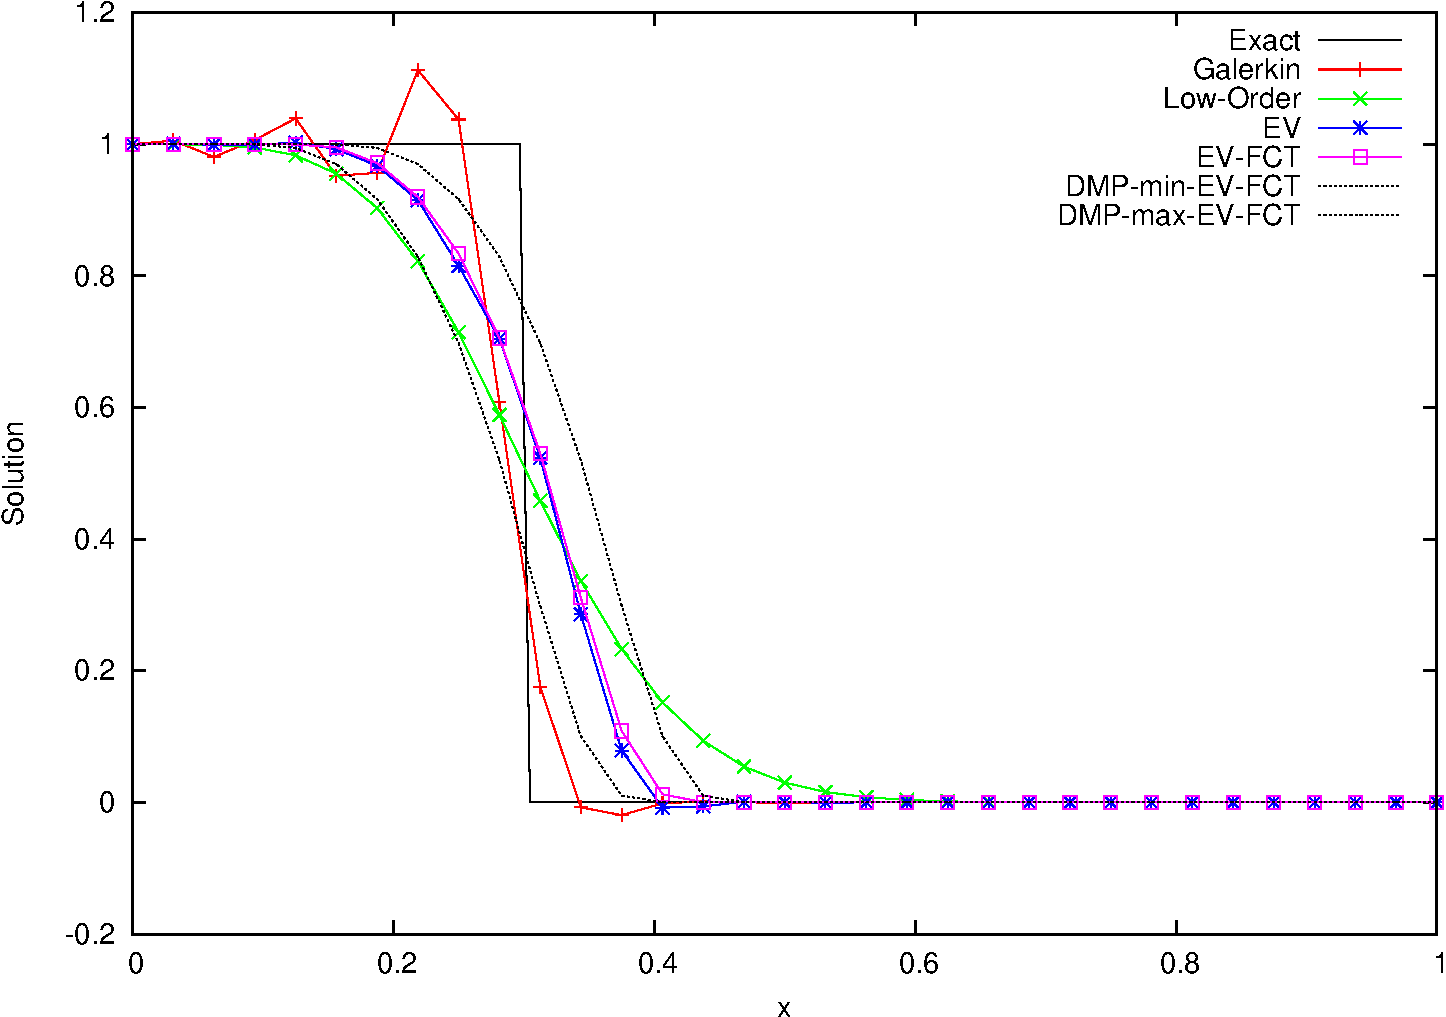
\includegraphics[width=\textwidth]{./figures/advection_FCT.pdf}

\end{frame}
%%%%%%%%%%%%%%%%%%%%%%%%%%%%%%%%%%%%%%%%%%%%%%%%%%%%%%%%%%%%%%%%%%%%%%%%%%%%%%%%%
\begin{frame}
\frametitle{Analytic Solution Bounds}

\begin{itemize}
  \item Solution bounds can be derived using the
    \hlorange{method of characteristics} (MoC):
  \begin{subequations}
  \begin{equation}
      W_i^{\textup{MoC},+}
        \equiv
          \solutionletter_{\max,i}^n
            e^{-\dt\reactioncoef_{\min,i}}
            + \frac{\scalarsource_{\max,i}}
              {\reactioncoef_{\min,i}}
            (1 - e^{-\dt\reactioncoef_{\min,i}}) \eqc
  \end{equation}
  \begin{equation}
      W_i^{\textup{MoC},-}
        \equiv
          \solutionletter_{\min,i}^n
            e^{-\dt\reactioncoef_{\max,i}}
            + \frac{\scalarsource_{\min,i}}
              {\reactioncoef_{\max,i}}
            (1 - e^{-\dt\reactioncoef_{\max,i}}) \eqp
  \end{equation}
  \begin{equation}
    \reactioncoef_{\max,i} = \max\limits_{\x\in\support_i}\reactioncoef(\x) \eqc
    \quad \scalarsource_{\max,i} = \max\limits_{\x\in\support_i}\scalarsource(\x) \eqc
  \end{equation}
  \end{subequations}
  \item Recall the low-order DMP bounds for explicit Euler:
  \begin{subequations}
      \begin{equation}
         \DMPbounds_i \equiv U_{\substack{\max\\\min},i}^n\left(
         1-\dt\bar{\reactioncoef}_i\right)
         + \dt\bar{\scalarsource}_i \eqc
      \end{equation}
      \begin{equation}
        \bar{\reactioncoef}_i \equiv
          \frac{\intSi\reactioncoef\testfunction_i\dvolume}
            {\intSi\testfunction_i\dvolume}
        \eqc \quad
        \bar{\scalarsource}_i \equiv
          \frac{\intSi\scalarsource\testfunction_i\dvolume}
            {\intSi\testfunction_i\dvolume}
      \end{equation}
  \end{subequations}
\end{itemize}

\end{frame}
